\section{Motoman Project Utilisation}
First thing to do is to create a ROS workspace where you will work.  So go to where you want to create your workspace and then create the workspace with a "src" folder inside. Then you go inside the "src" folder and initialize the catkin workspace.

\begin{lstlisting}
cd /where/you/want/your/workspace
mkdir -p my_workspace/src
cd my_workspace/src
catkin_init_workspace
\end{lstlisting}

Then download the motoman project repository. To do it you need to have the git program in your computer. To install git just type the following command.

\begin{lstlisting}
sudo apt-get install git
\end{lstlisting}

Then you need to download the repository. The "clone" command after the "git" command means you want to take the repository data and copy them into your current folder. So first go where your ros workspace and clone the github repository inside the "src" folder.  

\begin{lstlisting}
cd my_workspace/src
git clone https://github.com/Nishida-Lab/motoman_project.git
\end{lstlisting}

Then normaly a "motoman\_project" file would have been created in your "src" folder. The next step is to actually compile the project. To do this you need to use the "catkin\_make" command in the root of your workspace. But before that you need to be sure to have all the depedencies. 


\begin{lstlisting}
cd my_workspace
wstool init src src/motoman_project/dependencies.rosinstall
sudo apt-get install ros-indigo-industrial-msgs
sudo apt-get install ros-indigo-industrial-robot-simulator
sudo apt-get install ros-indigo-industrial-robot-client
sudo apt-get install ros-indigo-ros-controllers
rosdep install -i --from-paths src
catkin_make
\end{lstlisting}

After compiling everything (it could take some time!) you will be able to use the project. A simple test is to launch one of the launch file of the project. First you need to source the workspace to be sure that you can use the ROS command associated to your project.

\begin{lstlisting}
cd my_workspace
source devel/setup.bash
\end{lstlisting}

Then launch the empty environment with motoman inside by the following command.

\begin{lstlisting}
cd my_workspace
source devel/setup.bash
roslaunch motoman_gazebo sia5_empty_world.launch
\end{lstlisting}
\begin{figure}
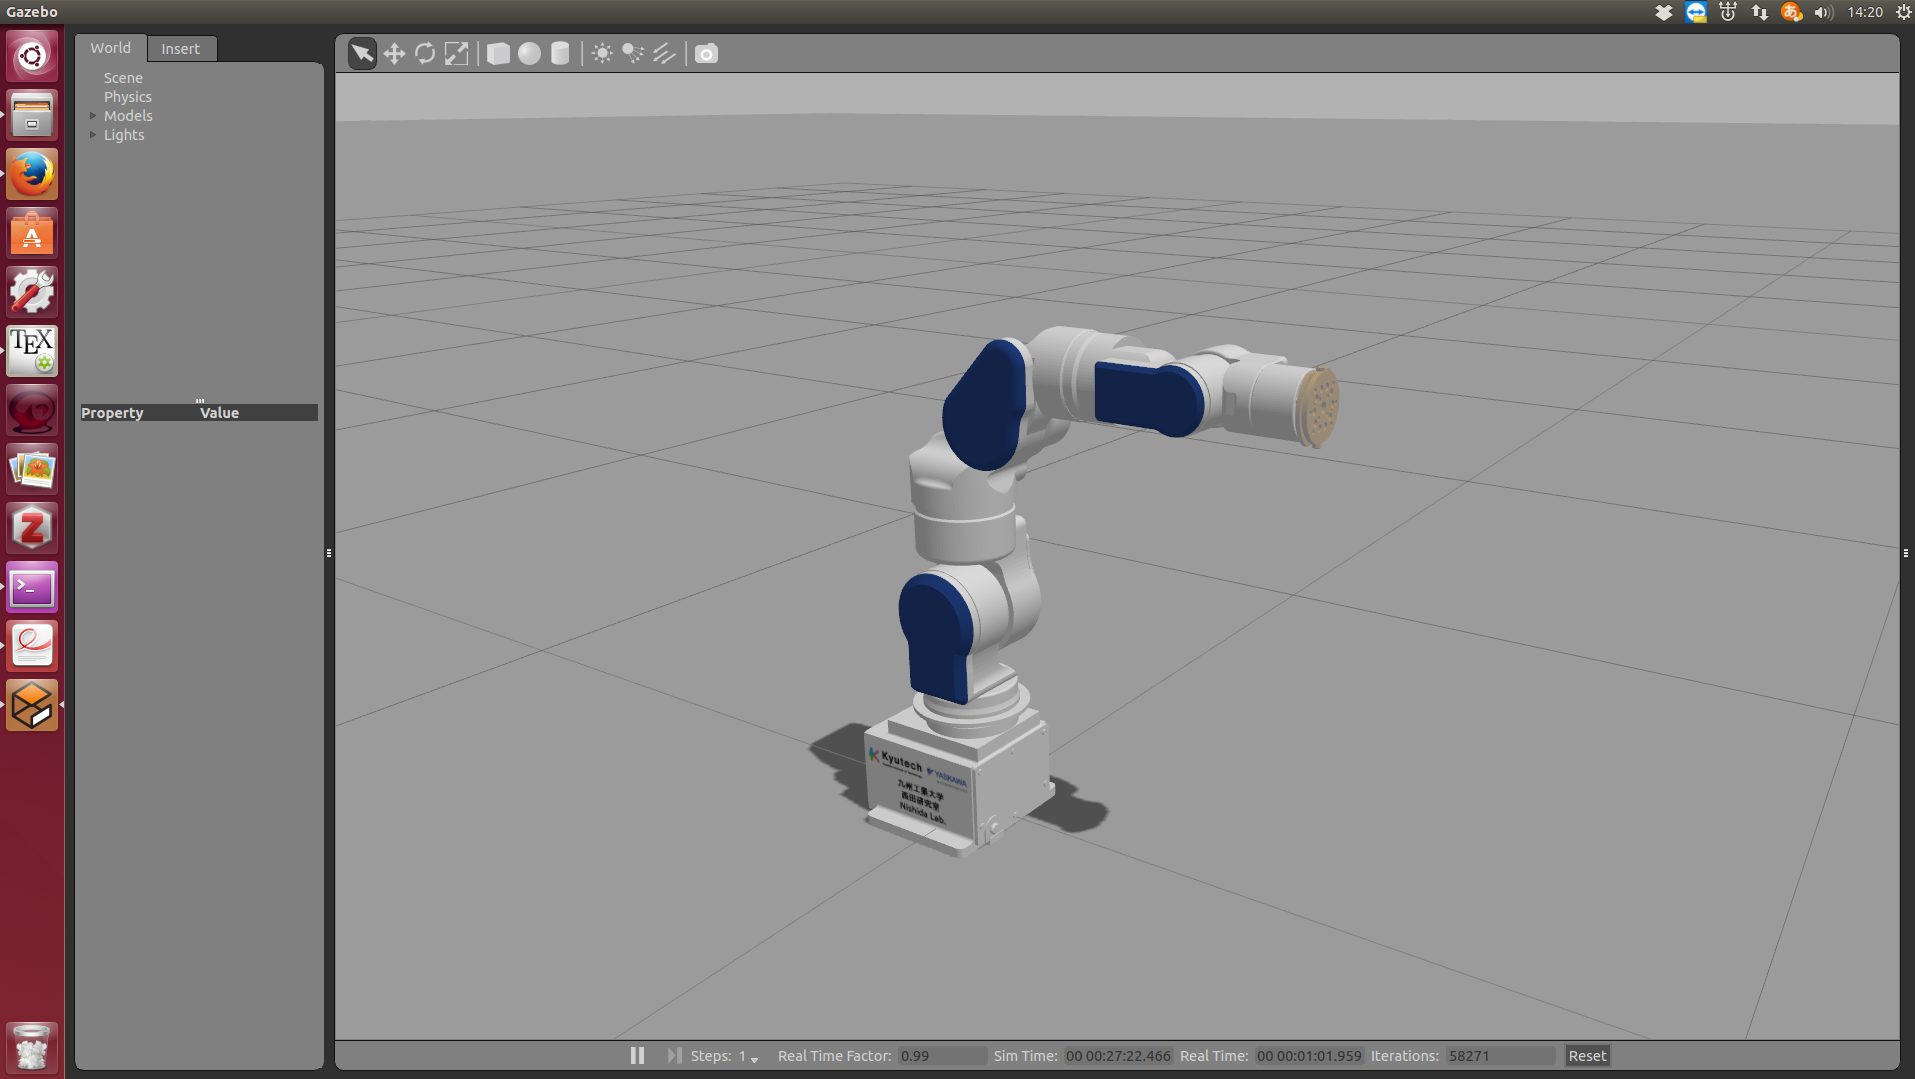
\includegraphics[width=8cm]{images/utilisation/launch_gazebo.png}
\centering
\label{fig:launch_gazebo}
\caption{Yo}
\end{figure}
You should normally have the gazebo software begin to run and you can soon see the motoman robot sia5 inside your screen like in Figure \ref{fig:launch_gazebo}.
